\subsection{Bildegjenkjenning}

\subsection{Mekanisk Instalasjon}
Når flyet skal svinge er flyet avhenigig av å gjøre en roll.
Dette fører til at buken til flyet ikke lengre peker rett ned mot bakken.
Et kamera i en låst posisjon, vil i denne situasjonen kunne oppleve at
objektet det skulle ha i bildet forsvinner ut av bildekanten.
Ved å feste kameraet til en rigg som kan kompensesere for at flyet beveger
seg vil dette problemet kunne løses.

For å beskytte kameraet ble det bestemt at kameraet skal kunne
trekkes inn i flyet ved landing.
Siden målene på fullskala fly ikke er fremstilt fra Kongsberg ble det
bestemt å følge målene på modellen i presentasjonen sendt fra Kongsberg.
Denne viser at plassen inne i er maksimalt 10.5 cm i høyden og 7.2 cm i bredden.
Kravet for riggen ble dermed at den ikke kunne oppta større plass i bredde
og høyde enn dette med kameraet tilfestet.
Det ble antatt at det for modellens skyld kunne brukes et lite kamera,
på størrelse med et mobilkamera. Den andre grunnen til å bygge en liten rigg
er for å hindre at vekten blir for stor.

En servomotor er en inretning som lar en kontrolere og holde på en vinkelposisjon.
En servomotor er bygget opp av en elektrisk motor,
en vinkelsensor og en kontroll enhet.
Et signal påtrykkes inngangen og motoren begynner å gå.
Vinkelsensoren vil fortelle vinkelen og når vinkelen som koresponderer
til inngangssignalet er nådd vil motoren stoppe.
Vinkelsensoren oppfører seg derfor som en tilbakekobling som returenerer feilen

\subsection{Hardware}
For å kunne styre riggen er det nødvendig å ha en datamaskin ombord i flyet. Det finnes en rekke alternativer på dette området, men her vil Arduino og Raspberry Pi bli presantert. Hovedoppgaven til datamskinen blir å få data fra kameraet, og orientere riggen etter disse. I systemspesifikasjonene til Kongsberg blir presisert at det allerede finnes en ekstern GPU som tar av seg bildebehandling, men man kan også tenke seg en løsning for all funksjonalitet er samlet på en chip.

\paragraph{Arduino}
Arduino er en open-source utviklings platform basert på 8bit \textit{atMega328}. Bruksområdet er hovedsakelig mindre prosjekter. Kortet har 14 digtale porter, samt 6 analoge in-porter. 6 av de digitale portene kan sende PWM-signaler. Servomotorer bruker disse signalene, og det er derfor mulig å koble opp til 6 servoer til Arduino. 

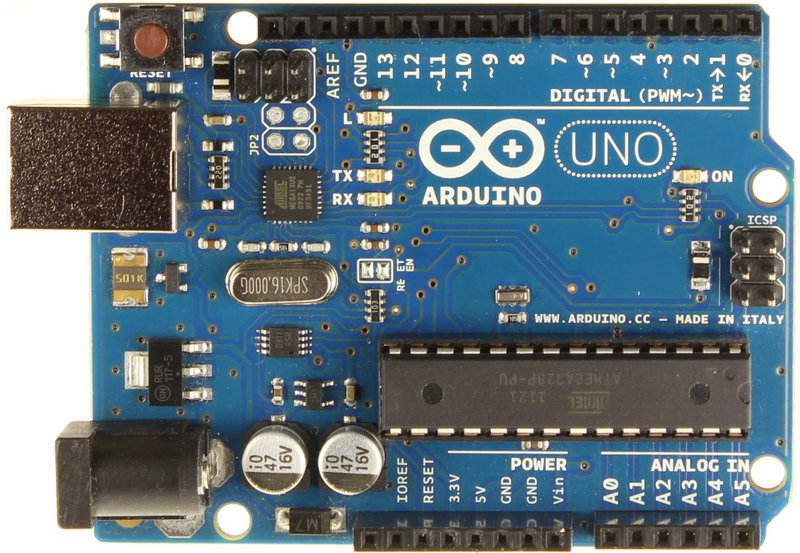
\includegraphics{img/arduinoBoard.jpg}
Arduino programmeres i C++, og programmene overføres til kortet via USB. USB-porten på kortet kan også benyttes som COM-port slik at Arduinoen kan ta inn eksterne kommandoer. Disse kommandoen kan for eksempel være vinkler som servomotorer skal innstilles til. På mikrokontrolleren er det også innstallert en bootlader som inneholder en rekke bilbioteker som gjør at abstraksjonsnivået blir høyere enn generell AVR-programmering. Dataregistre trenger ikke å endres når man vil åpne opp for en funksjon fordi bilibioteket vil håndtere dette. 

\paragraph{Raspberry Pi}
Raspberry Pi er en datamskin basert på 32-bit ARM-arkitektur. 

\begin{table}[h!]
\centering
\begin{tabular}{ |c |c |c| }
	\hline
   & Arduino & Raspberry Pi \\
	\hline
  CPU & 	ATmega328 & ARM1176JZF-S \\
  Klokkehastighet & 16 MHz & 700 MHz \\
	Minne & 32KB & 512MB\\ 
	CPU-størrelse & 8bit & 32bit\\
	i/o-porter & 14 & 8 \\
	PWN-porter & 6 & 1 \\
	Strømforbruk & 250mW & 3.5W\\
	Pris & \$26 & \$35 \\
	\hline  
\end{tabular}
\caption{Sammenligning mellom Arduino og Raspberry Pi}
\end{table}



